\chapter{Ejemplos.}
\label{chap:exa}

Ac\'a encontrar\'a algunos ejemplos de simulaciones realizadas con lpmd, en su ultima versi\'on estable.

%%%%%%%%%%%%%%%%%%%%%%%%%%%%%%%%%%%%%%%%%%%%%%%%%%%%%%%%%%%%%%%%%
%%%%%%%%%%%%%%%%%%%%%%%%%%%%%%%%%%%%%%%%%%%%%%%%%%%%%%%%%%%%%%%%%
\section{Ejemplos para LPMD}

Existen algunas l\'ineas dentro de cada ejemplo que al final poseen \verb|//|, lo que significa que la l\'inea no ha finalizado, sino que contin\'ua en la siguiente l\'inea.

\subsection{Celda de Ar de 108 \'atomos.}

A continuaci\'on una simulaci\'on de Ar con 108 \'atomos, en la cu\'al se realizan distintos escalamientos de temperatura. El ejemplo puede descargarlo completamente de,

\cajatx{http://wwww.gnm.cl/software/lpmd/examples/ar108-1.tgz}

Veamos el fichero de control.

\begin{multicols}{2}
\setlength{\columnseprule}{.5pt}
%\setlength{\columnsep}{20pt}
\begin{verbatim}
# System file of Ar gas 
# using LPMD
#
###################
#CELL and IN/OUT###
###################
cell crystal a=17.1191 b=17.1191 //
     c=17.1191 alpha=90.0 //
     beta=90.0 gamma=90.0

input module=lpmd file=Ar108.lpmd
output module=xyz file=output.xyz //
     each=20 level=0
###################
#GENERAL###########
###################
prepare replicate 1 1 1
prepare temperature 84
charge Ar 0.0
steps 5000
dumping file=ljargon.dump each=10000
periodic true true true

#Cargamos inmediatamente pressure
#para poder visualizar con monitor

use pressure
enduse

monitor start=0 end=5000 each=10 //
  properties=kinetic-energy, //
  potential-energy,total-energy, //
  pressure,volume output=monitor.dat
###################
#MODULES DEF#######
###################
use lennardjones as lj_Ar
    sigma 3.41
    epsilon 0.0103408
    cutoff 8.5
enduse

use beeman
    dt 10.0
enduse

use minimumimage
    cutoff 8.5
enduse
###################
#MOD APPLICATION###
###################
potential lj_Ar Ar Ar
integrator beeman
cellmanager minimumimage
\end{verbatim}
\end{multicols}


Corremos la simulaci\'on con 
\begin{verbatim}
  lpmd ljargon.control > salida.out
\end{verbatim}

\cajafi{ar108-1-energy.pdf}{Valores de la Energ\'ia para la simulaci\'on de Argon con 108 \'atomos.}{ar1081energy}

Podemos entonces ver algunos resultados de la simulaci\'on, por ejemplo la conservaci\'on de la energ\'ia a partir del fichero \verb|monitor.dat| que fue generado. Como se observa en la figura~\ref{fig:ar1081energy}. En un equipo moderno, la simulaci\'on no deber\'ia tardar m\'as all\'a de 40 segundos, puede observar los detalls de las cargas de los m\'odulos, asi como tambi\'en toda la informaci\'on de la simulaci\'on realizada en el archivo \verb|salida.out|. Junto con la finalizaci\'on de la simulaci\'on, se han generado los siguientes ficheros :

\begin{tabular}{lcl}\\
 monitor.dat &:& Guarda toda la informaci\'ond e monitoreo solicitada por la orden \verb|monitor|\\
&& del fichero de control. \\
 output.xyz &:& Salida de las posiciones at\'omicas de la celda de simulaci\'on. \\
 restore.dump &:& En caso de corte de luz o falla, sirve para reiniciar una simulaci\'on.\\
\end{tabular}

\subsection{Escalamiento de Temperatura.}

A continuacion veremos un ejemplo de escalamiento de temperatura, utilizando el rescalamiento cl\'asico, consistira en enfriar,de manera directa una muestra de Ar. El ejemplo puede encontrarse en:

\cajatx{http://wwww.gnm.cl/software/lpmd/examples/ar108-scalet.tgz}

El fichero de control, incorpora la carga del modulo tempscaling, modificando una muestra inicial de 5K de temperatura, hasta los 100K, como se puede apreciar, desde un paso intermedio de la simulaci\'on.

\begin{multicols}{2}
\setlength{\columnseprule}{.5pt}
\begin{verbatim}
# System file of Ar gas 
# using LPMD
#
###################
#CELL and IN/OUT###
###################
cell crystal a=17.1191 b=17.1191 //
     c=17.1191 alpha=90.0 //
     beta=90.0 gamma=90.0

input module=lpmd file=Ar108.lpmd
output module=xyz file=output.xyz //
     each=20 level=0
###################
#GENERAL###########
###################
prepare replicate 1 1 1
prepare temperature 84
charge Ar 0.0
steps 15000
dumping file=ljargon.dump each=10000
periodic true true true

#Cargamos inmediatamente pressure
#para poder visualizar con monitor

use pressure
enduse

monitor start=0 end=15000 each=10 //
  properties=kinetic-energy, //
  potential-energy,total-energy, //
  temperature,pressure,volume //
  output=monitor.dat
###################
#MODULES DEF#######
###################
use lennardjones as lj_Ar
    sigma 3.41
    epsilon 0.0103408
    cutoff 8.5
enduse

use beeman
    dt 10.0
enduse

use minimumimage
    cutoff 8.5
enduse

use tempscaling as TS
    from 5
    to 150
enduse
###################
#MOD APPLICATION###
###################
potential lj_Ar Ar Ar
integrator beeman
cellmanager minimumimage
apply TS start=5000 end=10000 each=200
\end{verbatim}
\end{multicols}

La aplicaci\'on del escalamiento de temperatura, genera un disen\~no autom\'atico para el decenso de la temperatura del sistema, en este caso vemos que el escalamiento se realiza de forma lineal y autom\'atica, partiendo en el paso 5000 a 5K y llegando en el paso 10000 a los 150K, donde la \textbf{inyecci\'on} de energ\'ia se aplica cada 200 pasos. Como se puede apreciar en la figura~\ref{fig:ar108scalet}

\cajafi{ar108-scalet.pdf}{Escalamiento de Temperatura.}{ar108scalet}

Muchas otras caracter\'isticas pueden ser observadas, a continuaci\'on una muestra de la celda entre 0 5000 pasos y luego de la termalizaci\'on se puede observar en la figuras~\ref{fig:ar108scaletemp-4000} y~\ref{fig:ar108scaletemp-15000}. Propiedades a partir de estas configuraciones \verb|xyz| pueden ser analizadas utilizando \textbf{lpmd-analyzer}.

\begin{figure}[!ht]
\centering
\subfigure[Configuraci\'on de Ar a los 4000 pasos de simulaci\'on.]
{
 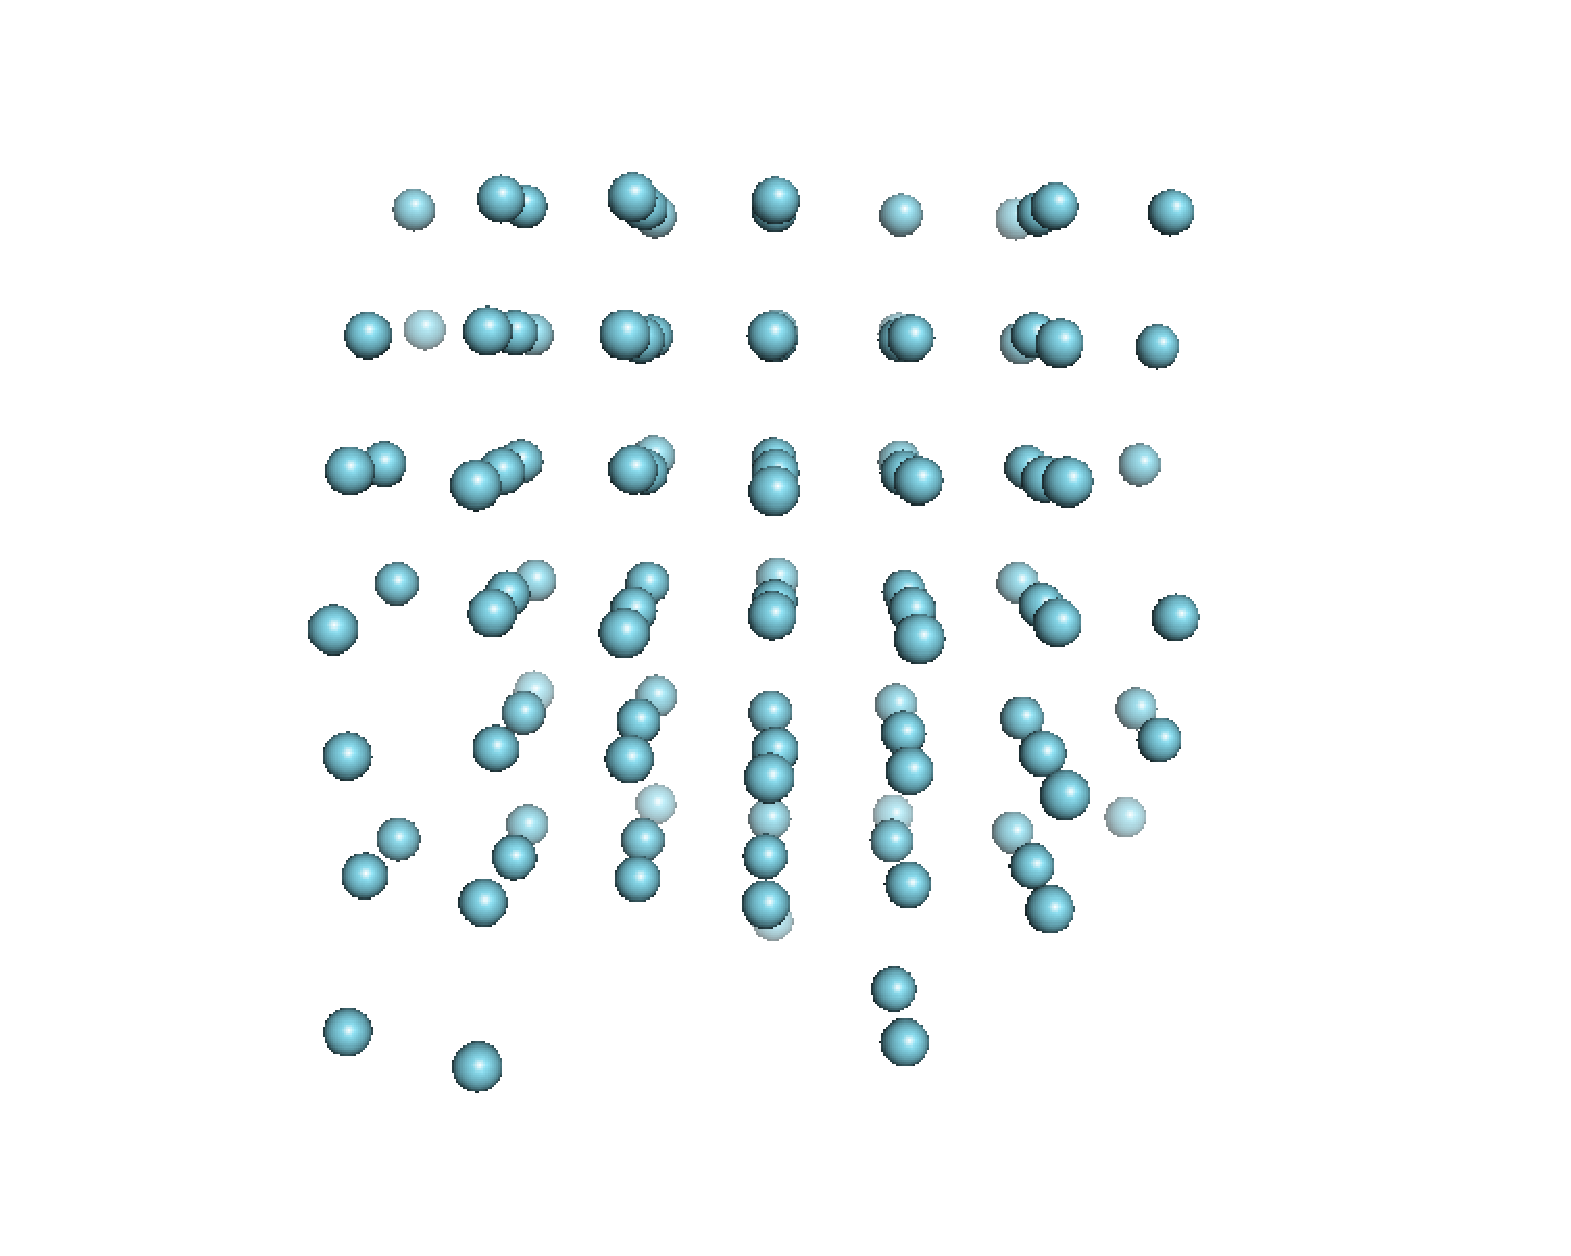
\includegraphics[scale=.25]{ar108scalet4000.pdf}
 \label{fig:ar108scaletemp-4000}
}
\subfigure[Configuraci\'on de Ar al finalizar la simulaci\'on.]
{
 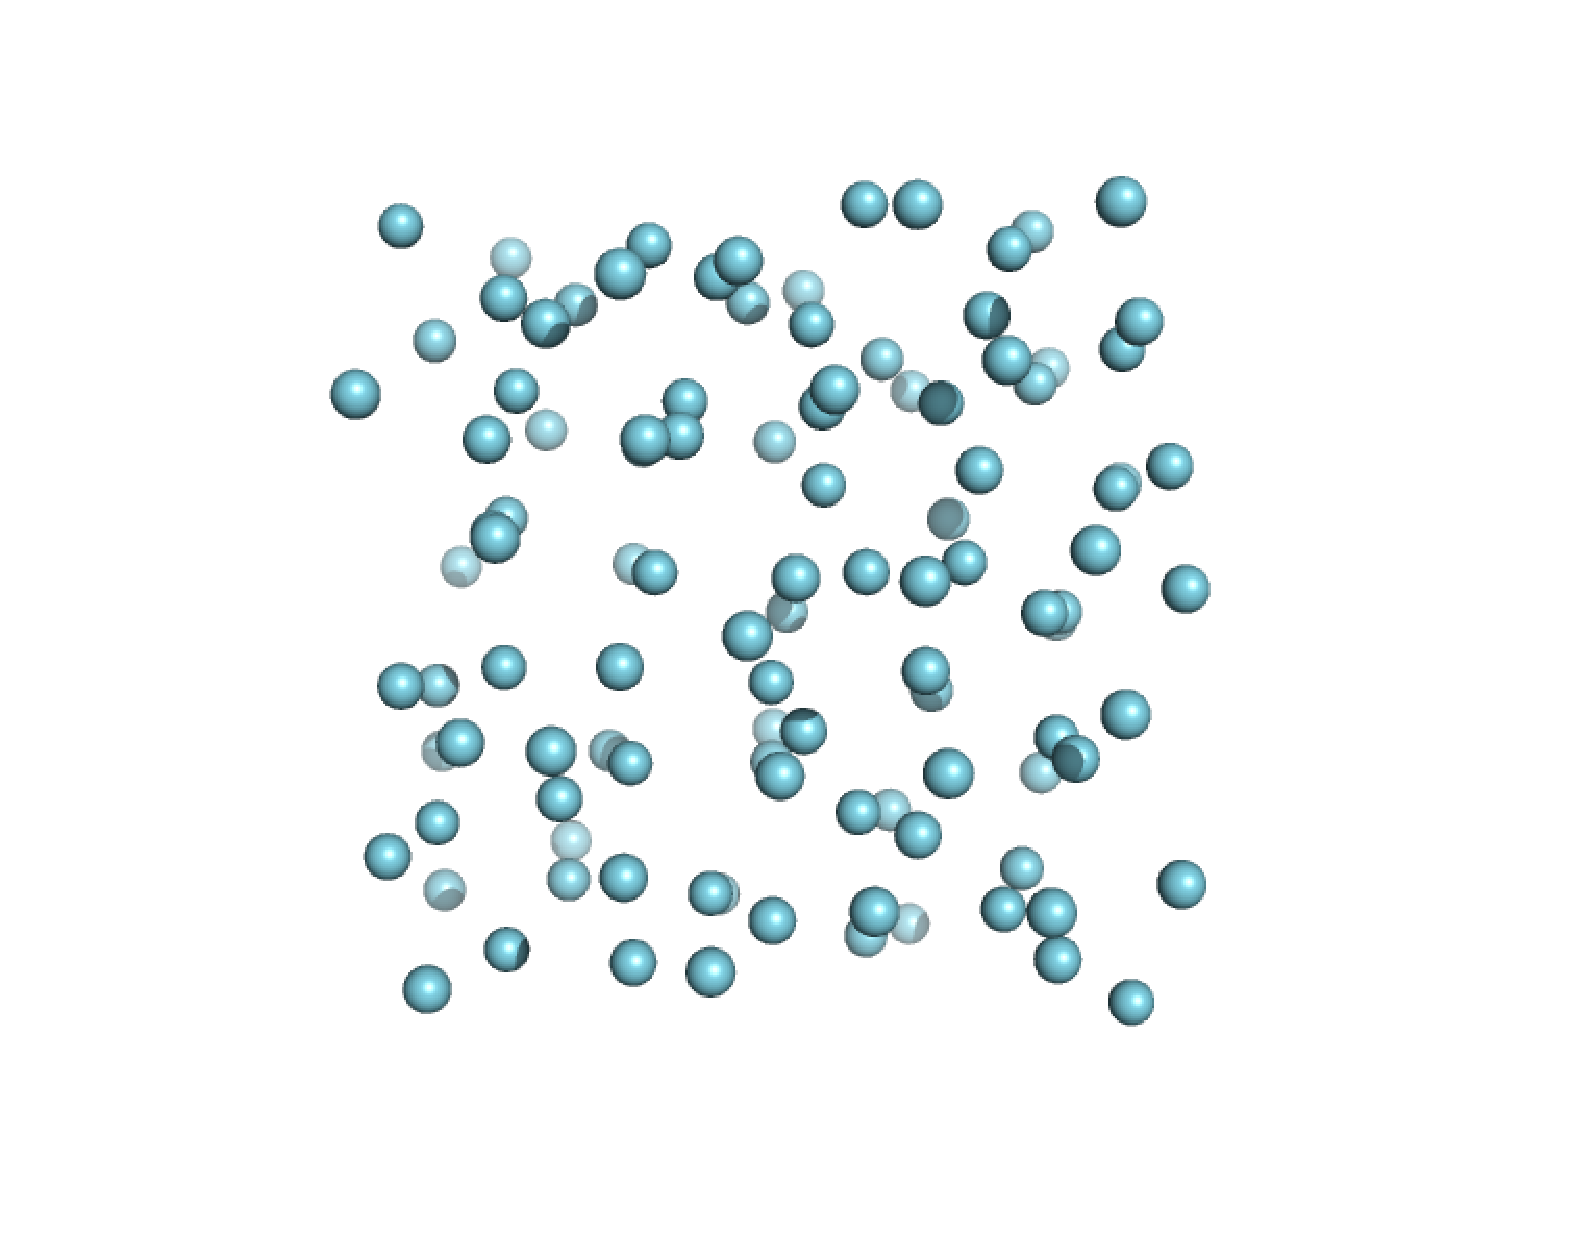
\includegraphics[scale=.25]{ar108scalet15000.pdf}
 \label{fig:ar108scaletemp-15000}
}
\caption{Distintos pasos de una simulaci\'on de din\'amica molecular de 108 \'atomos de Argon.}
\label{fig:ar108scaltemp}
\end{figure}

Adem\'as de este escalamiento de temperatura cl\'asico, \lpmd posee dentro de sus plugins otros termostatos, refierase al cap\'itulo\ref{chap:modulos}

\subsection{Escalamiento de Celda.}

Modificaremos las caracter\'isticas de la celda durante la simulaci\'on, para ello haremos uso del m\'odulo cellscaling, y luego veremos como se modifica la presi\'on del sistema, junto con la temperatura, el ejemplo esta disponible en

\cajatx{http://wwww.gnm.cl/software/lpmd/examples/ar108-scalec.tgz}

De manera similar a la anterior, se carga un modulo que modifica una propiedad de nuestro sistema, para llevarlo a las condiciones deseadas. En el siguiente fichero de control, se ve como se escala una celda.

\begin{multicols}{2}
\setlength{\columnseprule}{.5pt}
\begin{verbatim}
# System file of Ar gas 
# using LPMD
#
###################
#CELL and IN/OUT###
###################
cell crystal a=17.1191 b=17.1191 //
     c=17.1191 alpha=90.0 //
     beta=90.0 gamma=90.0

input module=lpmd file=Ar108.lpmd
output module=xyz file=output.xyz //
     each=20 level=0
###################
#GENERAL###########
###################
prepare replicate 1 1 1
prepare temperature 84
charge Ar 0.0
steps 15000
dumping file=ljargon.dump each=10000
periodic true true true

#Cargamos inmediatamente pressure
#para poder visualizar con monitor

use pressure
enduse

monitor start=0 end=15000 each=10 //
  properties=kinetic-energy, //
  potential-energy,total-energy, //
  temperature,pressure,volume //
  output=monitor.dat
###################
#MODULES DEF#######
###################
use lennardjones as lj_Ar
    sigma 3.41
    epsilon 0.0103408
    cutoff 8.5
enduse

use beeman
    dt 10.0
enduse

use minimumimage
    cutoff 8.5
enduse

use cellscaling as CS
    axis all
    percent 2
    constant true
enduse
###################
#MOD APPLICATION###
###################
potential lj_Ar Ar Ar
integrator beeman
cellmanager minimumimage
apply CS start=5000 end=10000 each=200
\end{verbatim}
\end{multicols}

Podemos ver entonces, como cambia la presi\'on y el volumen durante la simulaci\'on en las figuras~\ref{fig:ar108scalecpres} y~\ref{fig:ar108scalecvol}, con estos datos, uno puede obtener distintos tipos de propiedades mec\'anicas de los materiales en estudio, por ejemplo m\'odulo de \textit{Bulk}.

\begin{figure}[!ht]
\centering
\subfigure[Cambio de Presi\'on en el tiempo.]
{
 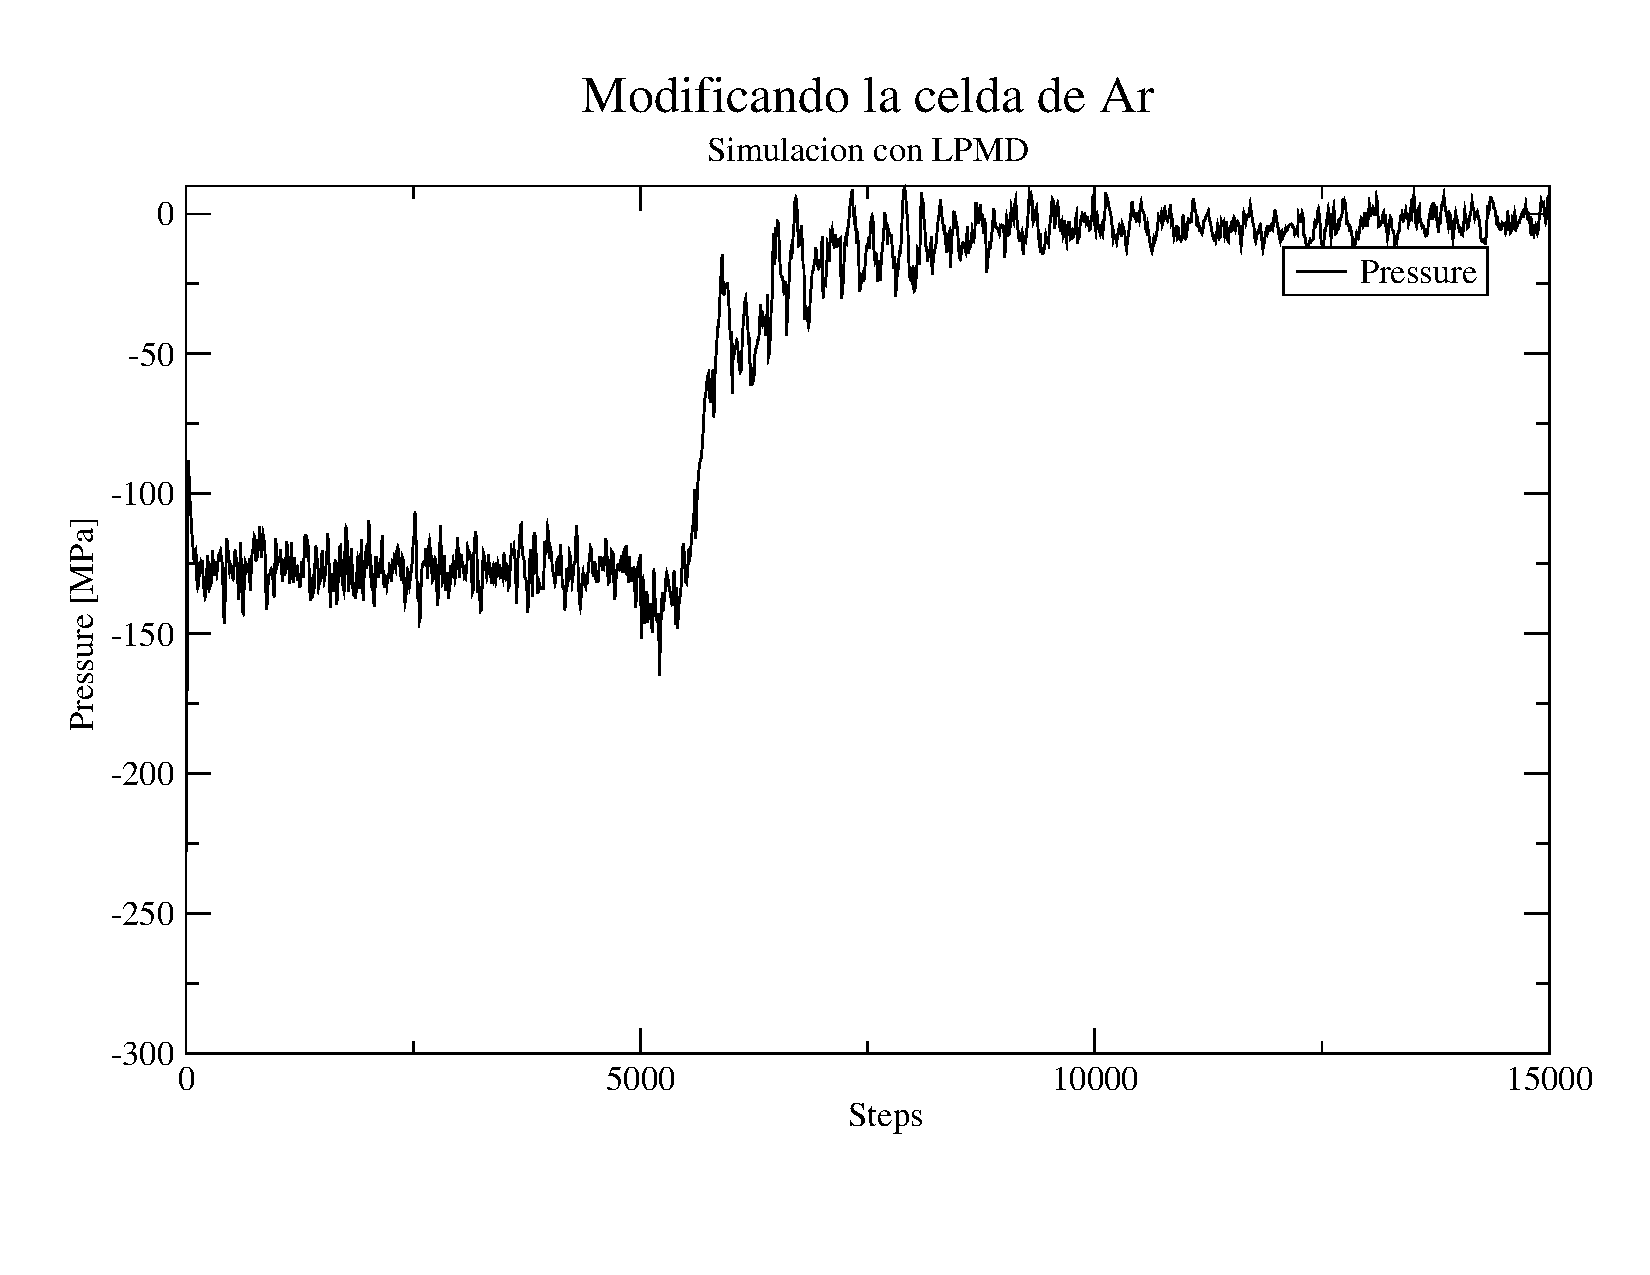
\includegraphics[scale=.25]{ar108scalecpres.pdf}
 \label{fig:ar108scalecpres}
}
\subfigure[Cambio de vol\'umen de la celda durante la simulaci\'on.]
{
 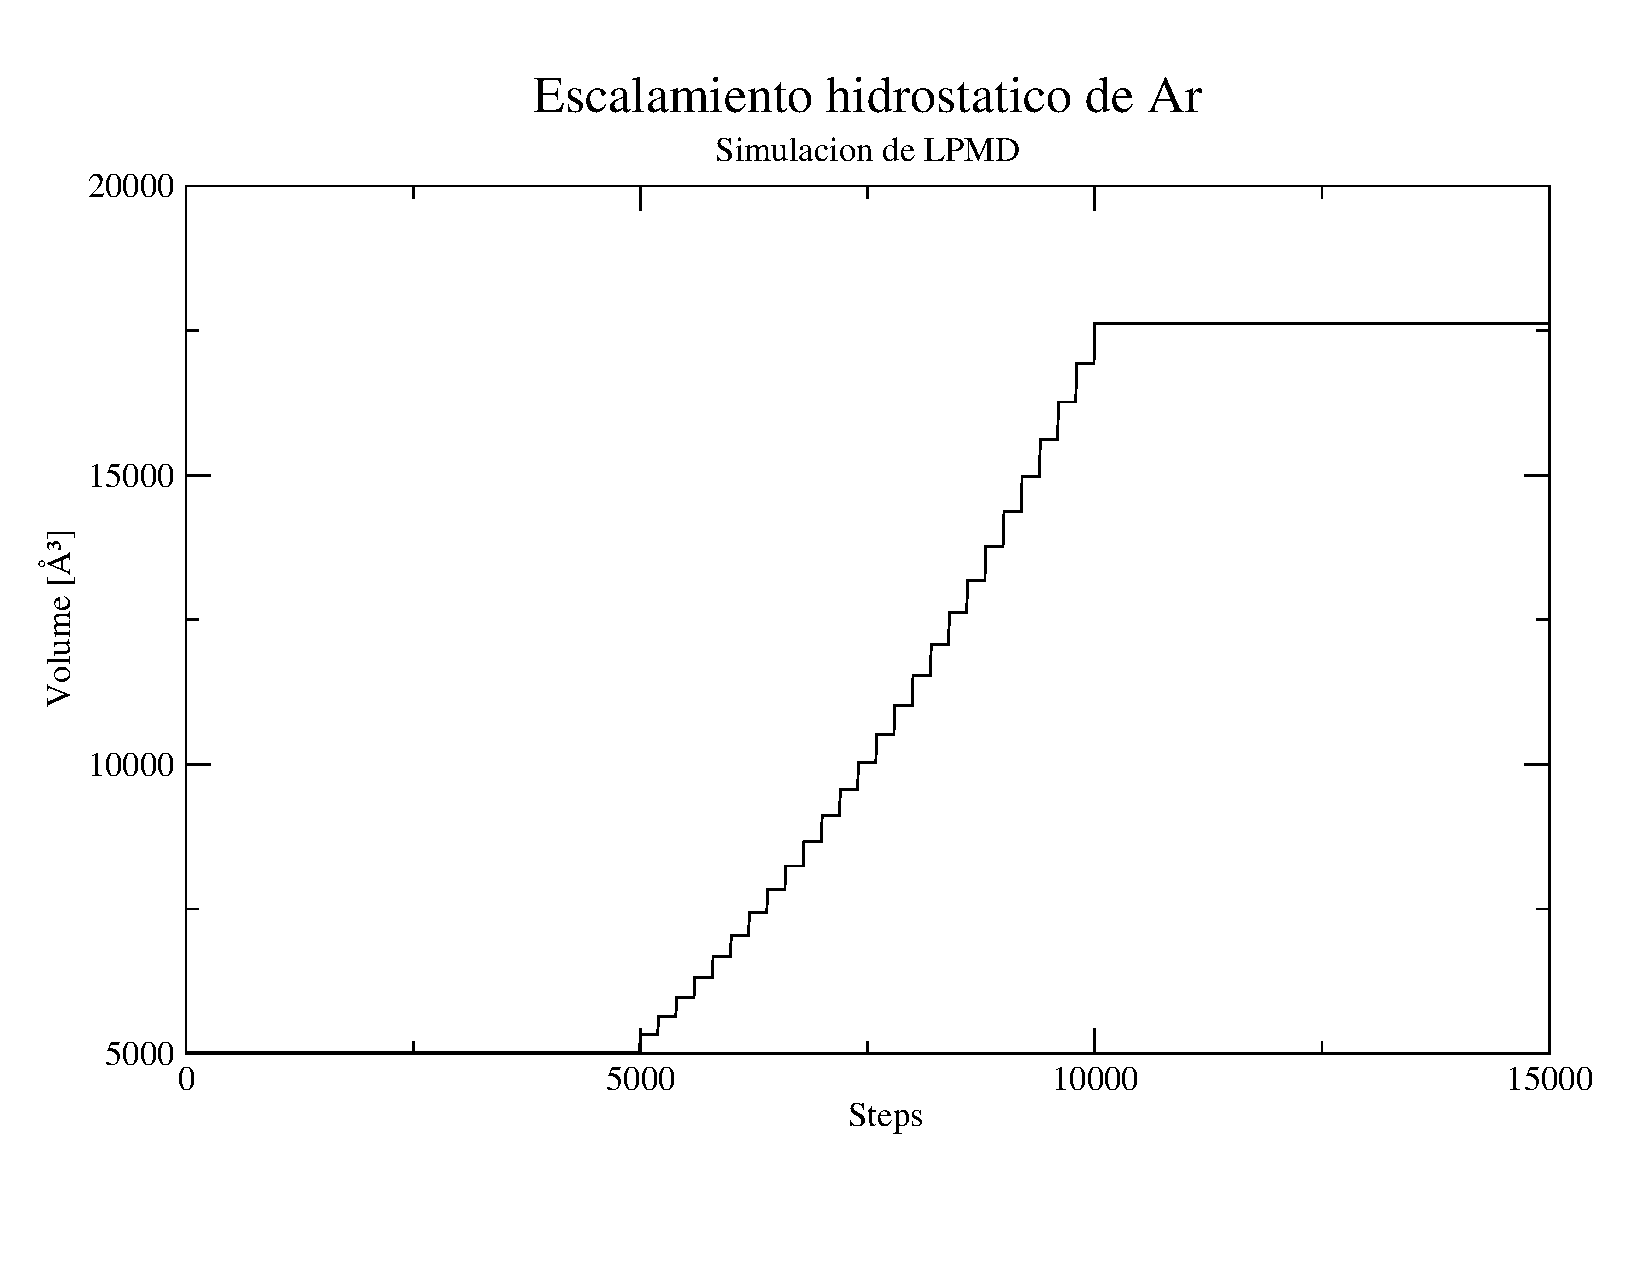
\includegraphics[scale=.25]{ar108scalecvol.pdf}
 \label{fig:ar108scalecvol}
}
\caption{Distintas propiedades del sistema, obtenidas durante la simulaci\'on.}
\label{fig:ar108scalec}
\end{figure}



\subsection{Calculando Propiedades durante la Simulaci\'on.}

A continuaci\'on, realizaremos un procedimiento simple de din\'amica molecular, pero esta vez, con una celda de Oro, sobre la cual calcularemos propiedades, durante la simulaci\'on. En este caso veremos, la \textit{funci\'on radial de distribuci\'on}, \textit{distribuci\'on angular} y \textit{n\'umero de coordinaci\'on}, un ejemplo de esto se puede encontrar en:

\cajatx{http://wwww.gnm.cl/software/lpmd/examples/au-prop.tgz}

\begin{multicols}{2}
\setlength{\columnseprule}{.5pt}
\begin{verbatim}

#Ejemplo de Oro!.

\end{verbatim}
\end{multicols}

en una maquina standard, no deber\'ia tardar mas de  ....  minutos. Las propiedades calculadas se pueden observar en la figura.

\subsection{Multiples corridas con bash.}

Haremos a continuaci\'on un peque\~no estudio de un gas de Ar a distintas temperaturas, para ello nos respaldaremos de los flags del comando \lpmd para poder modificar variables a partir de un fichero de control, relizaremos un estudio de la \textit{funci\'on de distribuci\'on de pares} para argon bajo distintas temperaturas.

\subsection{Generando ficheros pov para crear pel\'iculas.}

Fue uno de los primeros \textit{approach} a lo que a m\'odulos de visualizaci\'on se refiere, su intenci\'on es generar, a partir de la simulaci\'on, un set de ficheros \verb|pov| para un posterior renderizado y creaci\'on de peliculas, animaciones o simplemente imagnes de alta calidad.

\subsection{Cambiando el integrador durante la simulaci\'on.}

Una caracter\'istica de \lpmd es poder cambiar el integrador, durante la simulaci\'on, esto es utilizado en un ejemplo a continuaci\'on que puede descagar en:

\cajatx{http://wwww.gnm.cl/software/lpmd/examples/int-change.tgz}

\subsection{Multiples Monitor}

La informaci\'on en \lpmd puede ser \textbf{subdividida} seg\'un los requerimientos mismos del usuario a la hora de monitorear caracter\'isiticas propias de la celda de simulaci\'on. En este ejemplo, se guarda la informaci\'on de las energ\'ias, la celda y presiones, en tres ficheros distintos, para un an\'alisis mucho mas simple.

\cajatx{http://wwww.gnm.cl/software/lpmd/examples/multimon.tgz}

\subsection{Multiples Output}

Se puden guardar m\'as de un tipo de formato de dalida, lo que da distintas funcionalidades, sin la necesidad de convertir ntre los formatos, por ejemplo, los \verb|xyz| son mas utilizados para analizar, en cambio los \verb|lpmd| son m\'as portables por su caracter\'isticas de ser posiciones fraccionarias.

\cajatx{http://wwww.gnm.cl/software/lpmd/examples/multiout.tgz}

\subsection{Calculo de Modulo de Bulk}

En este ejemplo, se calcula el m\'odulo de Bulk para Au modificando el tama\~no de la celda de forma hidrostatica durante la simulaci\'on, para as\'i obtener directamente las presiones.

%%%%%%%%%%%%%%%%%%%%%%%%%%%%%%%%%%%%%%%%%%%%%%%%%%%%%%%%%%%%%%%%%
%%%%%%%%%%%%%%%%%%%%%%%%%%%%%%%%%%%%%%%%%%%%%%%%%%%%%%%%%%%%%%%%%
\section{Ejemplos LPMD-ANALYZER}

\subsection{Calculando funci\'on radial de distribuci\'on.}

\subsection{Calculando distribucion angular}

\subsection{Dos tipos de N\'umero de Coordinaci\'on}

\subsection{Distribuci\'on de velocidades}

\subsection{Autocorrelaci\'ond e velocidades}

%%%%%%%%%%%%%%%%%%%%%%%%%%%%%%%%%%%%%%%%%%%%%%%%%%%%%%%%%%%%%%%%%
%%%%%%%%%%%%%%%%%%%%%%%%%%%%%%%%%%%%%%%%%%%%%%%%%%%%%%%%%%%%%%%%%
\section{Ejemplos LPMD-CONVERTER}

\subsection{De un formato a otro}

\subsection{Formatos \'utiles}
